\documentclass{tufte-handout}

\title{Session 14}

\author[Pepe García]{Pepe García}

%\date{28 March 2010} % without \date command, current date is supplied

%\geometry{showframe} % display margins for debugging page layout

\usepackage{graphicx} % allow embedded images
  \setkeys{Gin}{width=\linewidth,totalheight=\textheight,keepaspectratio}
  \graphicspath{{../img/}} % set of paths to search for images
\usepackage{listings}  % for code
\usepackage{amsmath}  % extended mathematics
\usepackage{booktabs} % book-quality tables
\usepackage{units}    % non-stacked fractions and better unit spacing
\usepackage{multicol} % multiple column layout facilities
\usepackage{lipsum}   % filler text
\usepackage{fancyvrb} % extended verbatim environments
  \fvset{fontsize=\normalsize}% default font size for fancy-verbatim environments
\usepackage{xcolor}   % for colors

\definecolor{codegreen}{rgb}{0,0.6,0}
\definecolor{codegray}{rgb}{0.5,0.5,0.5}
\definecolor{codepurple}{rgb}{0.58,0,0.82}
\definecolor{backcolour}{rgb}{1,1,1}

\lstdefinestyle{mystyle}{
    backgroundcolor=\color{backcolour},
    commentstyle=\color{codegreen},
    keywordstyle=\color{magenta},
    numberstyle=\tiny\color{codegray},
    stringstyle=\color{codepurple},
    basicstyle=\ttfamily\footnotesize,
    breakatwhitespace=false,
    breaklines=true,
    captionpos=b,
    keepspaces=true,
    numbersep=5pt,
    showspaces=false,
    showstringspaces=false,
    showtabs=false,
    tabsize=4
}

\lstset{style=mystyle}

% Standardize command font styles and environments
\newcommand{\doccmd}[1]{\texttt{\textbackslash#1}}% command name -- adds backslash automatically
\newcommand{\docopt}[1]{\ensuremath{\langle}\textrm{\textit{#1}}\ensuremath{\rangle}}% optional command argument
\newcommand{\docarg}[1]{\textrm{\textit{#1}}}% (required) command argument
\newcommand{\docenv}[1]{\textsf{#1}}% environment name
\newcommand{\docpkg}[1]{\texttt{#1}}% package name
\newcommand{\doccls}[1]{\texttt{#1}}% document class name
\newcommand{\docclsopt}[1]{\texttt{#1}}% document class option name
\newenvironment{docspec}{\begin{quote}\noindent}{\end{quote}}% command specification environment

\begin{document}

\maketitle% this prints the handout title, author, and date

\begin{abstract}
  \noindent
  In this \textbf{Async session} you'll go over a series of exercises to learn how to
  model data depending on the problem at hand.

  Being able to select the correct datatype for each use case is one of the most
  important skills we'll need to program efficiently.
\end{abstract}

%\printclassoptions

\section{Exercises}\label{sec:exercises}

In this series of exercises we´ll see how different problems require different
data structures.

There are solutions for this problems in the \hyperref[sec:solutions]{Solutions}
section, but try to work on these examples without looking at them beforehand.

\pagebreak

\subsection{DNS}\label{sec:dns}

In this first example we'll try to model what a DNS server does.

\begin{marginfigure}%
  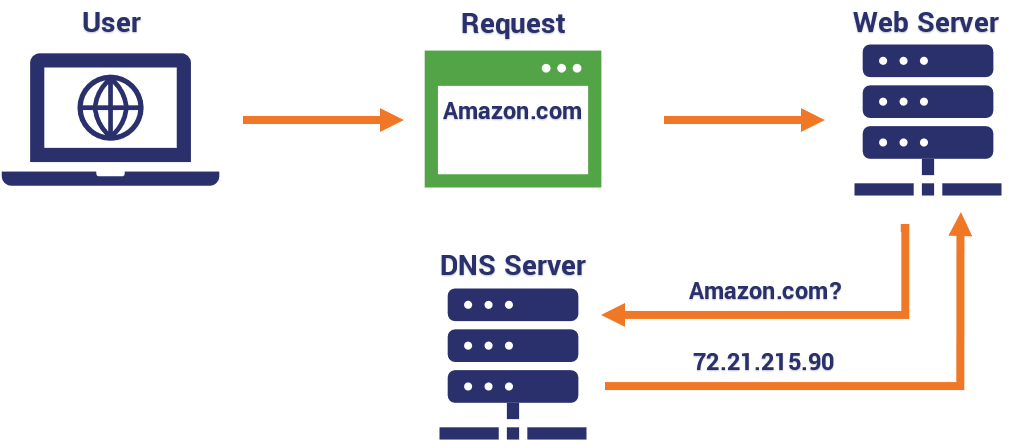
\includegraphics[width=\linewidth]{dns.png}
  \caption{\newthought{the Domain Name System} is the subsystem of the Internet in charge of
    translating from domain names to IP addresses.  Each computer connected to the
    Internet has an IP address associated so that other computers can refer to it.
    These addresses look like \textbf{102.43.250.21}, making it fairly hard to
    remember them all.\\Luckily, \textbf{DNS} allows us to map domain names, such as
    \textbf{google.com} to IP addresses like \textbf{102.43.250.21}}
  \label{fig:marginfig}
\end{marginfigure}

For this exercise we need to first create a \textit{database} that contains the
mappings from domain names to ip addresses.  This \textit{database} we'll save
it in a variable called \Verb|database| and should contain the following
mappings:

\begin{center}
  \begin{tabular}{||c c||}
    \hline
    \textbf{Domain name} & \textbf{IP address} \\ [0.5ex]
    \hline\hline
    amazon.com           & 10.32.23.111        \\
    \hline
    google.com           & 10.255.23.111       \\
    \hline
    wordpress.com        & 253.32.23.31        \\
    \hline
  \end{tabular}
\end{center}

Once you have your \Verb|database| created, define a function called
\Verb|resolve_dns| that allows you to translate from a domain name to a IP
address, and if the domain name is unknown, returns \Verb|None|.

\pagebreak

\subsection{Matrices}\label{sec:matrices}

Matrices mathematical objects composed by smaller elements and distributed in
rows and columns.

\begin{figure}
  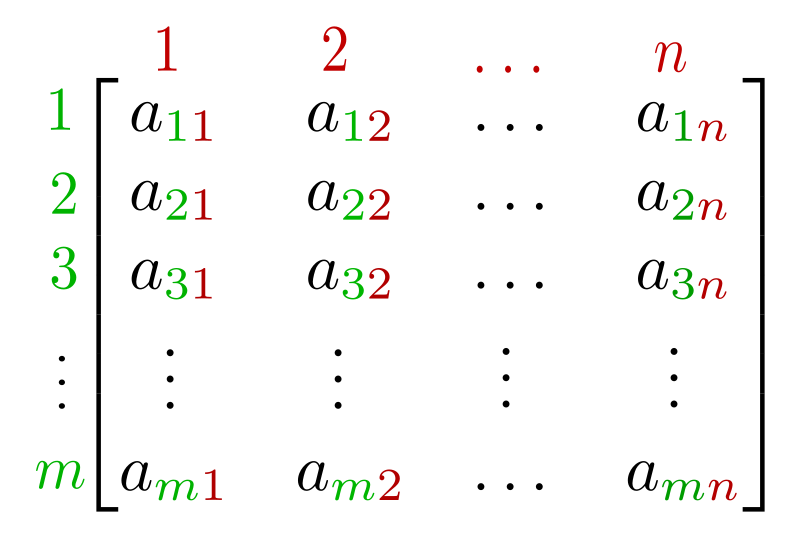
\includegraphics{Matrix.png}
  \caption{This image shows a $m * n$ matrix.}
  \label{fig:matrix}
\end{figure}

In order to add matrices together we need to sum elements position wise. Given

\[
  A & =
  \begin{pmatrix}
    1 & 2 & 3 \\
    2 & 3 & 4 \\
    3 & 4 & 5 \\
  \end{pmatrix}
\]

and

\[
  B & =
  \begin{pmatrix}
    4 & 5 & 6 \\
    5 & 6 & 7 \\
    6 & 7 & 8 \\
  \end{pmatrix}
\]

Then:

\[
  A + B & =
  \begin{pmatrix}
    5 & 7  & 9  \\
    7 & 9  & 11 \\
    9 & 11 & 13 \\
  \end{pmatrix}
\]

We calculate each position in the sum matrix as follows:

\[
  (A + B)_i_j = A_i_j + B_i_j
\]

Now, try to implement matrix addition using Python.  First we need to model
matrices in a way that allows us to use them.

Let's create two variables, \Verb|a| and \Verb|b| that contain the same matrices
we've declared above.

Afterwards, create a function \Verb|matrix_addition(a, b)| that performs matrix
addition.  This function should return the sum matrix.

\pagebreak

\section{Solutions}\label{sec:solutions}

\subsection{Solution for \hyperref[sec:dns]{DNS}}


\begin{marginfigure}%
  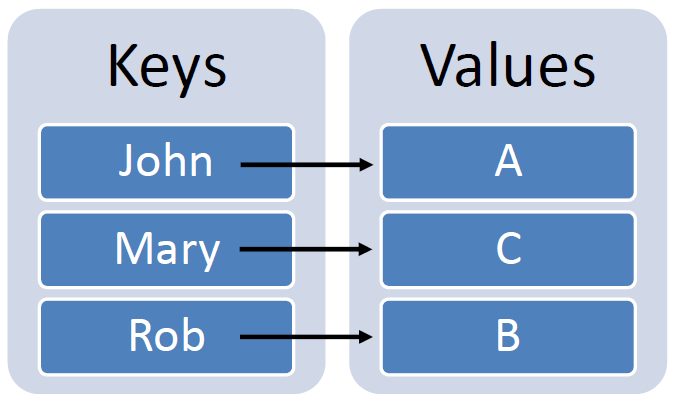
\includegraphics[width=\linewidth]{dict.png}
  \caption{In this exercise it makes sense to use a \textbf{dictionary} because
    we're mapping between two sets.  Domain names and IP addresses. \\
    Each one of the entries in our \textit{database} becomes an entry in our
    \textbf{dictionary}, with a \textbf{key} for the domain name and a
    \textbf{value} for the IP address}
  \label{fig:marginfig}
\end{marginfigure}

\begin{lstlisting}[language=Python]
database = {
  "amazon.com": "10.32.23.111",
  "google.com": "10.255.23.111",
  "wordpress.com": "253.32.23.31"
}

def resolve_dns(domain):
    # if ... in  checks if an element (domain in this case) exists in
    # the keys of a dictionary
    if domain in database:
        # If it exists, we return it
        return database[domain]
    else:
        # Otherwise, we return None, the empty value
        return None
\end{lstlisting}

\pagebreak

\subsection{Solution for \hyperref[sec:matrices]{Matrices}}

\begin{marginfigure}%
  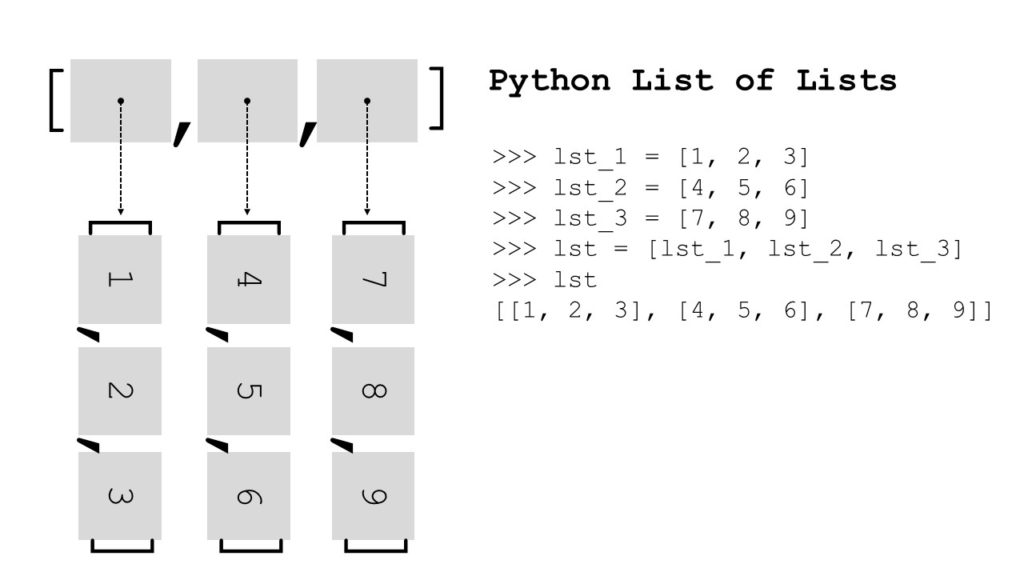
\includegraphics[width=\linewidth]{listoflist.jpg}
  \caption{
    For this problem, it makes sense to use \textbf{lists of lists} to represent matrices.
    Lists can be contained within other lists in Python.
    \\
    Since the size of a matrix is unbounded, they can start at zero rows and columns
    up to an infinite number of rows and columns, it makes sense to use lists, which
    allow us to make them grow as much as we need.
  }
  \label{fig:marginfig}
\end{marginfigure}

\begin{lstlisting}[language=Python]
  A = [
    [1, 2, 3],
    [2, 3, 4],
    [3, 4, 5]
  ]
  
  B = [
    [4, 5, 6],
    [5, 6, 7],
    [6, 7, 8]
  ]
  
  def matrix_addition(a, b):
      # We start with an empty list for our solution matrix
      solution = []
  
      # i is the index for our rows
      i = 0

      # here we're iterating over all rows
      while i < len(a):
          # We start by creating an empty row
          solution.append([])
          
          # j is the index for our columns
          j = 0

          # here we're iterating over all columns in a row
          while j < len(a[i]):
              # At this point we use the method we know from matrix addition
              # to sum this position on a and b matrices.
              solution[i].append(a[i][j] + b[i][j])
              j = j + 1
          i = i + 1
  
      return solution
\end{lstlisting}

\end{document}
